\documentclass{article}
\usepackage[utf8]{inputenc}
\usepackage{amsmath}
\usepackage[nopatch]{microtype}
\usepackage{booktabs}
\usepackage{indentfirst}
\usepackage{graphicx}
\graphicspath{ {./images/} }
\usepackage{blindtext}

\title{Security Risk Assesment In IoT Based Smart Houses}

\author{Adithan Kumaresan}

\begin{document}


\maketitle

\begin{abstract}
\textbf{The new and problematic age of shrewd residential
bundles in light of
Internet of Things (IoT) is essentially controlled and dispersed.
Homes are Beginning to become filled with interconnected devices on the internet which makes the house unsafe as it is susceptible to external attack and data stealing.}
\end{abstract}


\section{Introduction}
Internet has changed human’s lifestyles by way of
presenting anytime, anywhere connectivity with all and
sundry. As many advancements in generation has been come the sensors, processors, transmitters, receivers, and so on.
Are now available in very cheap price. Hence these all
matters can be utilized in our daily lifestyles. 
This means the idea of owning a smart house has become very feasable to the common man.
\begin{figure}
\begin{center}
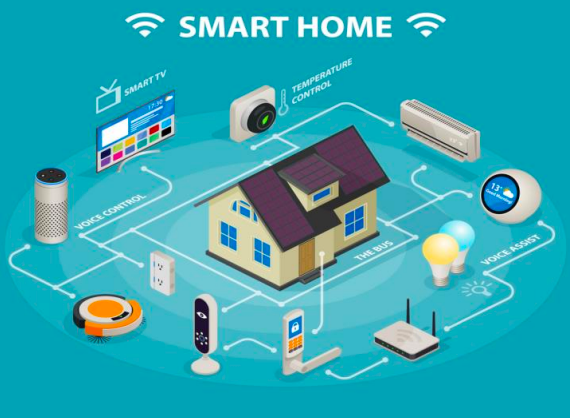
\includegraphics[width=6cm]{smarthome.png}
\end{center}
\caption{Smart Home Components}
\end{figure}
\section{IoT in Smart Homes}
\subsection{Example : Apple EcoSystem}
keen home or robotized home could be established on a phase
or focus focuses that control clever devices and mechanical
assemblies. For instance, using Apple's Home Kit, producers
can have their home things and decoration obliged by an
application in iOS devices, for instance, the iPhone and the
Apple Watch. This could be a dedicated application or iOS
neighborhood applications, for instance, Siri. 
\subsection{Application}
a versatile application
where he/she:
\begin{itemize}
    \item 1. can turn on or off LED lights and screen the
condition of the LED.
    \item 2. can bolt and open entryways through servo engines
and screen if the entryways are bolted or opened.
    \item 3. can screen if the entryways are shut or opened
through IR sensors.
    \item 4. is advised through email if the entryway is left open for a really long time.
    \item 5. is advised of who entered through the entryway as
the camera catches the face picture and send it to him/her by
means of email.
    \item 6. is informed through email if the fire identifier
distinguishes smoke.
    \item 7. is ready to control the observation vehicle from
anyplace to screen his/her home.
\end{itemize}
\section{Application of Smart Home Systems}
\subsection{Structure}
Smart systems give you a previously unavailable picture of how things work in your household
\subsection{Sensors and actuators}
There are sensors for a broad collection of
employments, for example, estimating temperature,
moistness, light, fluid, and fuel and figuring out development
or commotion.
The IoT gadgets geared up with sensors
will cross about as government and the ones implanted with
actuators will move about as entertainers.
Actuators are the strategies for the way the
eager system can in all fact get matters carried out in fact.
There are mechanical actuators, as an instance, siphons and
electrical engines or digital actuators, for example, electric
powered switches.
\subsection{Architechture}
A Layer Architechtural Model is used in the architechture of a iot based smart home system

\begin{center}
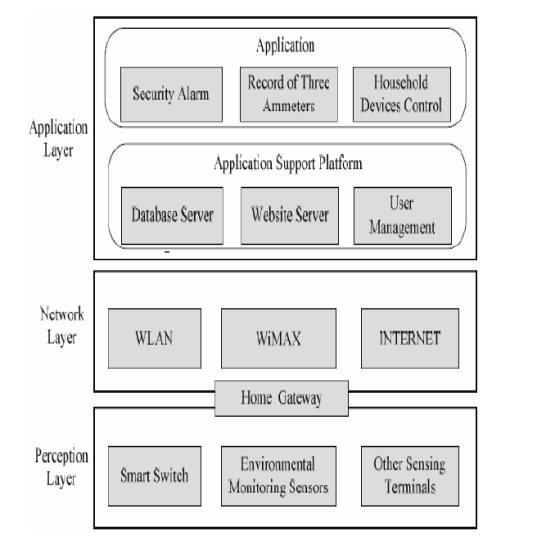
\includegraphics[width=6cm]{Architechture.png}
\end{center}

\section{Risk Assesment}
\subsection{OCTAVE Allegro technique}
Basic records
advantages for the savvy home can be prominent, alongside
its vulnerabilities and capacity risks.
The goal of a
hazard appraisal is to recognize the contemporary framework
and condition, to recognize dangers and their consequences
through investigation of the records collected.
If any abnormality is sensed by the model it will alert the user by email and text throught the raspberry pi.
\subsection{Parts Used}
\begin{itemize}
    \item Raspberry pi2
    \item IR sensor
    \item Net digital camera
    \item OpenCV software
\end{itemize}
These items are interconnected to form the smart risk assesing system to protect the house from any iminent cyber attack.
\begin{center}
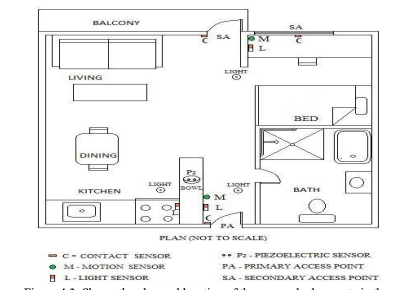
\includegraphics[width=7cm]{Sensor Deployment.png}
\end{center}
\section{Conclustion}
\textit{There are a couple
of issues found in IoT and Smart Homes. New advances
could help with constraining some of them.
The introduction of Iot Systems in out houses is a new advancement to technology but it brings along with it big risks but these risks can be mitigated by using safety mmodels such as the OCTAVE Allegro technique and other such solutions.}
\section{References}
\begin{itemize}
    \item \textbf{Research Paper on Internet of Things based
upon Smart Homes with Security Risk
Assessment using OCTAVE Allegro}
by \textit{Ahmad Bilal Zia1} and \textit{Ms. Kshamta Chauhan}
    \item https://www.digiteum.com/iot-smart-home-automation/
    \item https://www.ibm.com/blogs/internet-of-things/sensors-smart-home/
    \item https://www.trendmicro.com/vinfo/us/security/news/internet-of-things/inside-the-smart-home-iot-device-threats-and-attack-scenarios
\end{itemize}
\end{document}
